\documentclass[a4paper, onecolumn, 10pt]{article}

\usepackage[english]{babel}
\usepackage[latin1]{inputenc}
\usepackage[T1]{fontenc}

\usepackage{float} % For controlling figure positions
\usepackage{etoolbox} % For using conditionals
\usepackage{amsthm} % For using \begin{proof}...
\usepackage{amsfonts}
\usepackage{amssymb}
\usepackage{amsmath}
\usepackage{fancybox}
\usepackage{color}
\usepackage{cite}
\usepackage{url}

\usepackage{graphicx}
\graphicspath{ {../img/} }

\usepackage{authblk}

\usepackage[draft,colorinlistoftodos]{todonotes} % Use disable instead of draft to hide todo notes

\title{Neutral competition among prey promotes chaos in two-level food webs}
\author[1]{Pablo Rodr�guez-S�nchez \thanks{pablo.rodriguezsanchez@wur.nl}}
\author[1]{Egbert van Nes \thanks{egbert.vannes@wur.nl}}
\author[1]{Marten Scheffer \thanks{marten.scheffer@wur.nl}}

\affil[1]{Department of Aquatic Ecology, Wageningen University, The Netherlands}

\usepackage[switch]{lineno}

%\linenumbers

\begin{document}

\maketitle

\begin{abstract}
\label{sec:Abstract}
Neutral competition can be interpreted as a limit case between dominant intraspecific competition and dominant interspecific competition. Using a numerical model of an ecosystem with two trophic levels, we explore the surroundings of this limit case, that is, weak non-neutral competition interactions. It is shown that, the closer the competition is to neutrality, the higher are the chances of the system to develop chaotic behaviour. The competitive exclusion principle, based in equilibrium assumptions, is thus less likely to be applicable to neutral ecosystems. As a result, these systems have more chances of holding a higher amount of coexisting species than non neutral ones.

\paragraph{}
\textit{Keywords}: population dynamics, competition models, neutral competition, biodiversity paradox, chaos.
\end{abstract}

%\clearpage
\tableofcontents
\listoftodos[TODOs]
%\clearpage

\section{Background}
\label{sec:Background} 

% Introductory paragraph
Fascination for biodiversity is one of the main motivations for studying ecology. Even very young children feel the joy of learning about different species, so no prior knowledge of biology seems to be a requirement for being sensitive to the amazing variety of life. Scientific knowledge increases this sense of wonder even more as there is a big mystery: why are there so many species?\todo{why are there so many species is not the complete paradox}
%TODO why are there so many species is for me not the complete translation of the paradox

% Introduction of the biodiversity paradox 
The mystery comes into scene together with the competitive exclusion principle\cite{Hardin1960}, sometimes referred to as Gause's law. This principle, which some authors trace back to Charles Darwin's \textit{On the origin of the species}\cite{Darwin1859}, is one of the classical keystones of ecology. The principle states that \textit{"for each niche only one species will dominate in the long run, out-competing the rest"}. Most competition models satisfy this principle, and it has been observed experimentally under laboratory conditions. On the other hand, complete exclusion rarely occurs in nature\cite{Huston1979}, being the huge biodiversity in Earth its most noticeable counterexample. This contradiction is known as the biodiversity paradox. The paradox can be carelessly (but poetically) rephrased as \textit{Why are there so many species if there are so few niches?}
%% Brief discussion about the alternative hypotheses
% Introduction and hypotheses based in non-autonomous systems
There are several hypotheses to explain the paradox. For instance, Hutchinson\cite{Hutchinson} reports his observations on two sympatric species of beetles competing for the same resource, but not simultaneously because of having different breeding seasons. In a later, influential paper\cite{Hutchinson1961}, Hutchinson proposes the possibility of ecosystems to be driven by external, time-dependent seasonal environmental changes. If the characteristic times of this environmental changes are fast enough, the ecosystem is prevented to reach an equilibrium. A pioneering quantitative discussion about ecosystems subject to periodically driven external perturbations can be found in \cite{Huston1979}.

% Introduction of chaotic dynamics
After the discovery of chaos\cite{Lorenz1963}, it has been shown that non-equilibrium ecosystems can arise as well under constant environmental conditions\cite{May1974}. More specifically, those ecosystems develop cyclic or chaotic dynamics instead of fixed points. Of course, chaotic dynamics can arise as well in seasonally changing environments in a food web (as, for instance the model with multiple predators studied in \cite{Dakos2009b}).

% Hypotheses based in spatial heterogeneity 
All the previous hypotheses refer to the time domain. Regarding the spatial dimension, the inhomogeneity of ecosystems, and the possibility of migration between them has been pointed out as another possible explanation of the paradox \cite{Tilman1994}.\todo[caption={Broken flow}]{Flow broken here}
%TODO according to Tobias, the flow is broken here. High risk of the reviewer stopping reading! 
% Why are all the previous explanations not sufficient?
% Why does neutrality deserve attention?

% Introduction of the neutral theory 
Another hypothesis deserving attention are that of neutral competition, whose better known exponent is \textit{Hubbell's neutral competition theory} \cite{Hubbell2001}. In neutral models, similar species inside an ecological community are assumed to have identical \textit{per capita} rates of birth, death, reproduction, etc. In those models, the long term differences between species are a result of random events. Despite its counter-intuitive and controversial foundations, neutral models have been successfully applied to populations of rainforest trees.
\todo{Cite Scheffer2006 and Yachi1999}
%TODO About reconciling (near) neutral and niche theroy, cite {Scheffer2006}
%TODO In neutral models the species can coexist because they are identical. But this is rather unrealistic, as species will for instance react differently to perturbations (response diversity Loreau Maybe introduced in this publcation (please check): Yachi, S. and M. Loreau. 1999. Biodiversity and ecosystem productivity in a fluctuating environment: The insurance hypothesis. Proceedings of the National Academy of Sciences of the United States of America 96:1463-1468 {Yachi1999}

%TODO We need to make this motivation stronger, something like this?:
%- Most of these theories include competition only
%- Predation is important in many ecosystems and involves often many species (for instance phytoplankton/zooplankton)
%- Multi-species predation may strongly increase the probablity of chaos (Dakos), and may thus contribute to the number of coexisting species.
%- Here we study if neutrally competing species in combination with multispecies predation may increase or decrease the probabiluty of chaos.
% Introduction to our contribution
\todo{Stronger motivation required}
In the present paper we explore the links between neutral competition and the type of long term dynamics exhibited. Using competition models with different degrees of heterogeneity, our simulations show that the likelihood of chaotic dynamics increases when heterogeneity at the competitors' trophic level is minimal. That is, that neutrality in combination with multiple predators may promote chaos.
\todo{Not clear motivation}
%TODO not clear why I want to study: the links between neutral competition and the type of long term dynamics exhibited

\section{Methods}
\label{sec:Methods}

\subsection{Model description}
\label{subsec:Model}
We focused our attention on food webs with two trophic levels, one of consumers and another of prey (see figure \ref{fig:Network}). The consumers predate on the prey, and the prey populations compete among each other for a common source of resources. 

\begin{figure}[h]
	\begin{center}
		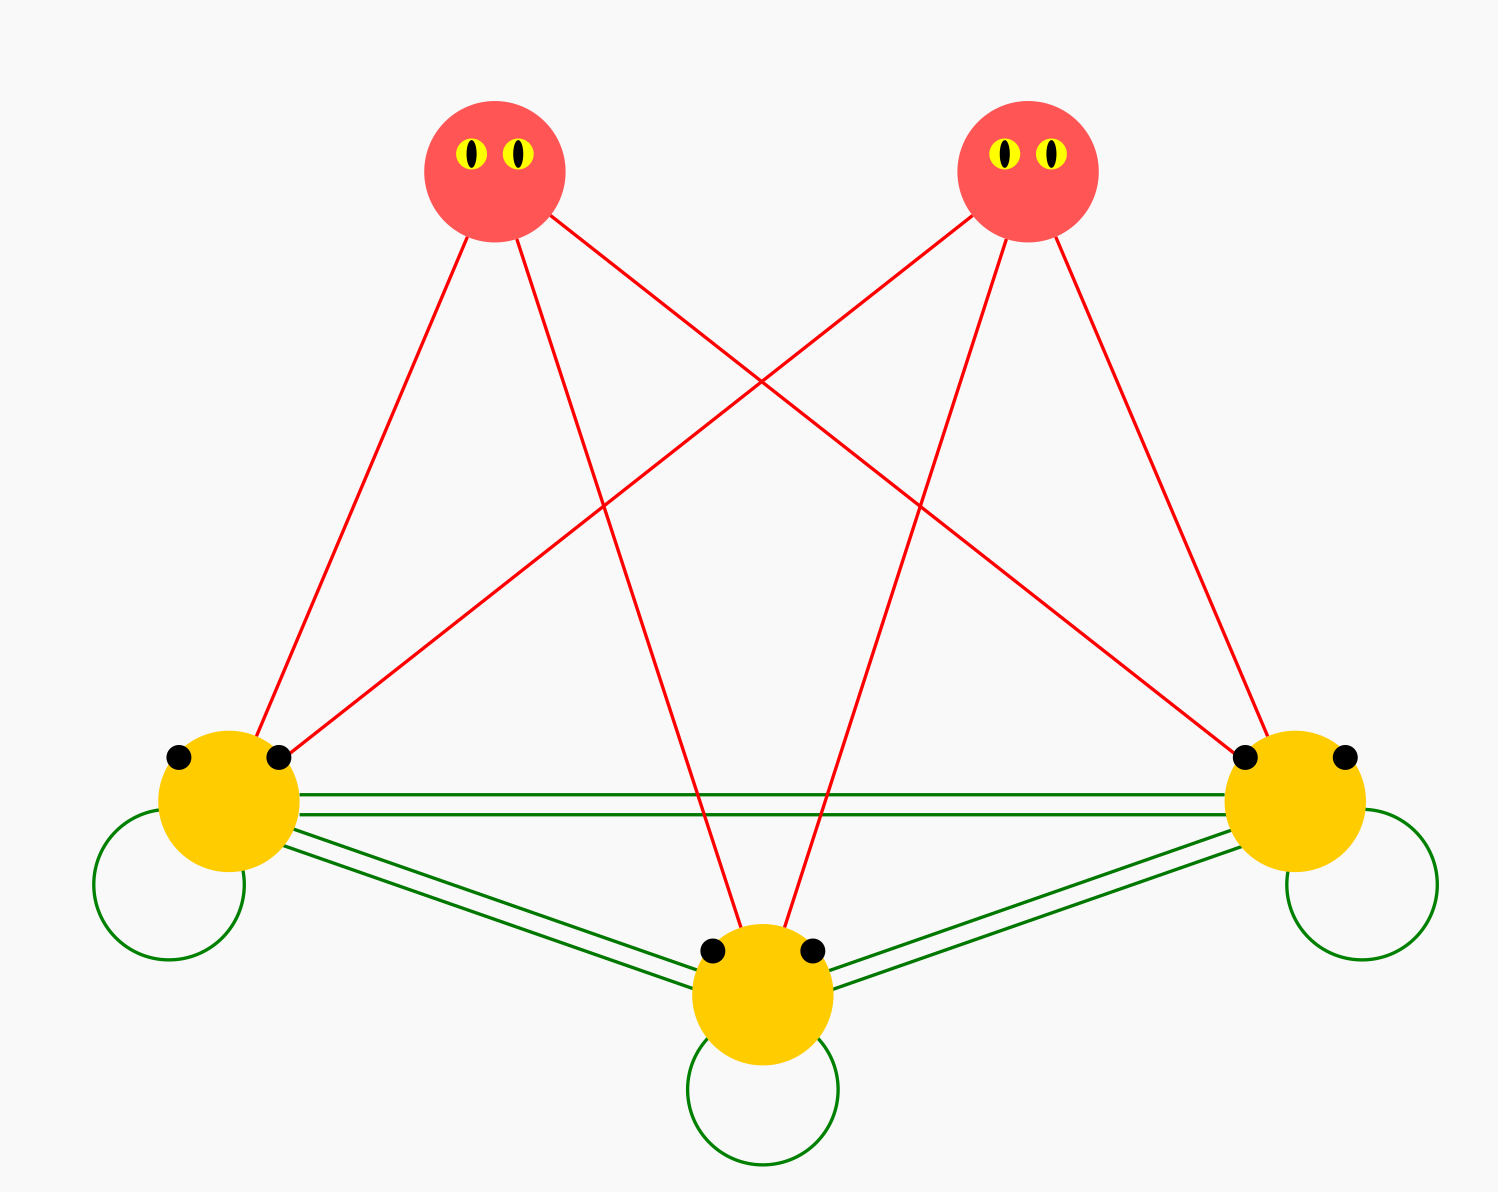
\includegraphics[width=0.7\columnwidth]{net.png}
	\end{center}
	\caption{Example with $2$ consumers and $3$ prey. Each one of the red links represents a predation interaction (coded in the matrix of predator preference coefficients, $ S $). Each green link represents a competition interaction (coded in the matrix of competition coefficients, $ A $). The closed green loops are related with carrying capacity (diagonal elements of $ A $) interpreted here as intra-species competition.}
	\label{fig:Network}
\end{figure}

% Description of the dynamics
The dynamics were modelled as a system of ordinary differential equations. We used the Rosenzweig-MacArthur predator-prey model \cite{Rosenzweig1963} generalized to a higher number of species \cite{Scheffer2004}. Our model is composed of $ n_P $ prey species and $ n_C $ consumer species. $ P_i(t) $ was used for accounting the size of the population of prey $ i $ at time $ t $, and $ C_j(t) $ for the population of consumer $ j $. When it is not explicitly stated, $ i $  runs from $ 1 $ to $ n_P $, and $ j $ from $ 1 $ to $ n_C $. The prey compete directly among themselves, while the consumers compete indirectly by sharing the same food. The consumers eat all kind of prey, but find some of them more preferable than others. All these interactions are summarized in figure \ref{fig:Network}. The overall structure looks like:

\begin{displaymath}
\label{eq:EquationInPseudocode}
	\begin{cases}
	\frac{d}{dt} \left( Prey \right) = Growth  - Predation + Immigration \\
	\frac{d}{dt} \left( Cons \right) = Feeding - Death \\
	\end{cases}
\end{displaymath}

%% Step-by-step description of each term
The growth term is modelled as a multispecies logistic growth. The strength of the competition between species $ i $ and $ k $ is given by the community matrix element $ A_{ik} $. So, for prey $ i $, we have:

\begin{equation}
\label{eq:Growth-Competition}
%\resizebox{.8 \columnwidth}{!}
%{
Growth_i  = r P_i \left( 1 - \frac{1}{K} \sum_{k=1}^{n_P} A_{ik} \cdot P_k \right)
%}
\end{equation}

A secondary source for prey's growth in our model will be a constant immigration term $ f $, representing immigration from neighboring areas. We introduce this term in order to avoid complete extinctions.

The predator preference for each prey species is given by $ S_{ij} $. That is, the matrix element $ S_{ij} $ represents the relative proportion of prey $ i $ in consumer's $ j $ \textit{menu}. Being a multispecies model, we can define an auxiliary variable $ V_j $ as a sum of the prey's populations weighted by the predator preference coefficients. Biologically, this represents the composition of the \textit{menu} of consumer $ j $:

\begin{equation}
\label{eq:MenuFunction}
	V_j(P) \equiv \sum_{k=1}^{n_P} S_{jk} \cdot P_k
\end{equation}

We hypothesized that the feeding term will be linear in $ C_j $. The dependency on $V_j$ happens through a Holling type II functional response with half saturation constant $ H $ in order to account for consumer satiation\cite{Edelstein-Keshet}.

\begin{equation}
\label{eq:Feeding}
	Feeding_j = e g C_j \frac{V_j}{V_j+H}
\end{equation}

$ e $ represents the assimilation efficiency of the predation. Thus, the effect of consumer $ j $ on all prey's populations is given by $ Feeding_j/e $. Knowing this, we can sum the effect of all consumers in the prey species $ i $ as follows:

\begin{equation}
\label{eq:Predation}
	Predation_i = g \sum_{k=1}^{n_C} \left(\frac{S_{ki}P_i}{V_k}\right) C_k F_{2}(V_j; H)
\end{equation}

Where the term inside the parentheses represents the relative proportion of prey species $ i $ inside "the menu" of predator $ k $, and $F_{2}$ is a shorthand for the Holling type II functional form introduced before. It is interesting to note that the way the predation and feeding terms are defined satisfies the following property:

\begin{equation}
\label{eq:Balance}
	\sum_{j=1}^{n_C} Feeding_j = e \sum_{i=1}^{n_P} Predation_i
\end{equation}

that is, all the deaths at the prey level are invested in the growth of consumers. For future clarity, it is a good idea to define the auxiliary function $ R_i $ as a summary of the effect of all consumers on prey $ i $:

\begin{equation}
\label{eq:PredationAux}
	R_i(P,C) \equiv \sum_{k=1}^{n_C} \left(\frac{S_{ki}P_i}{V_k(P)}\right) C_k F_{2}(V_k(P); H) 
\end{equation}

Putting all together, the dynamical system reads:

\begin{eqnarray}
\label{eq:SystemUnderStudy}
	\begin{cases}
	\dot{P_i} = r P_i \left( 1 - \frac{1}{K} \sum_{k=1}^{n_P} A_{ik} \cdot P_k \right) - g R_i(P,C) + f
	\\ 
	\dot{C_j} = e g C_j F_{2}(V_j(P); H) - l C_j
	\end{cases}
\end{eqnarray}

Depending on the parameters and the initial conditions, this system can give rise to three types of asymptotic behavior, each of them roughly corresponding to a different type of attractor. The easier one, corresponding to a stable point attractor, generates a constant species composition. Cyclic attractors give rise to periodically changing species composition. Beyond fixed points and cycle attractors, there is a wide variety of more complex possible behaviors. As a simplification, we'll refer to all them as chaotic. Chaotic behavior makes the species composition keep changing without reaching a fixed point nor giving rise to periodicity (see figure \ref{fig:TimeSeries}).

\begin{figure}
	\begin{center}
		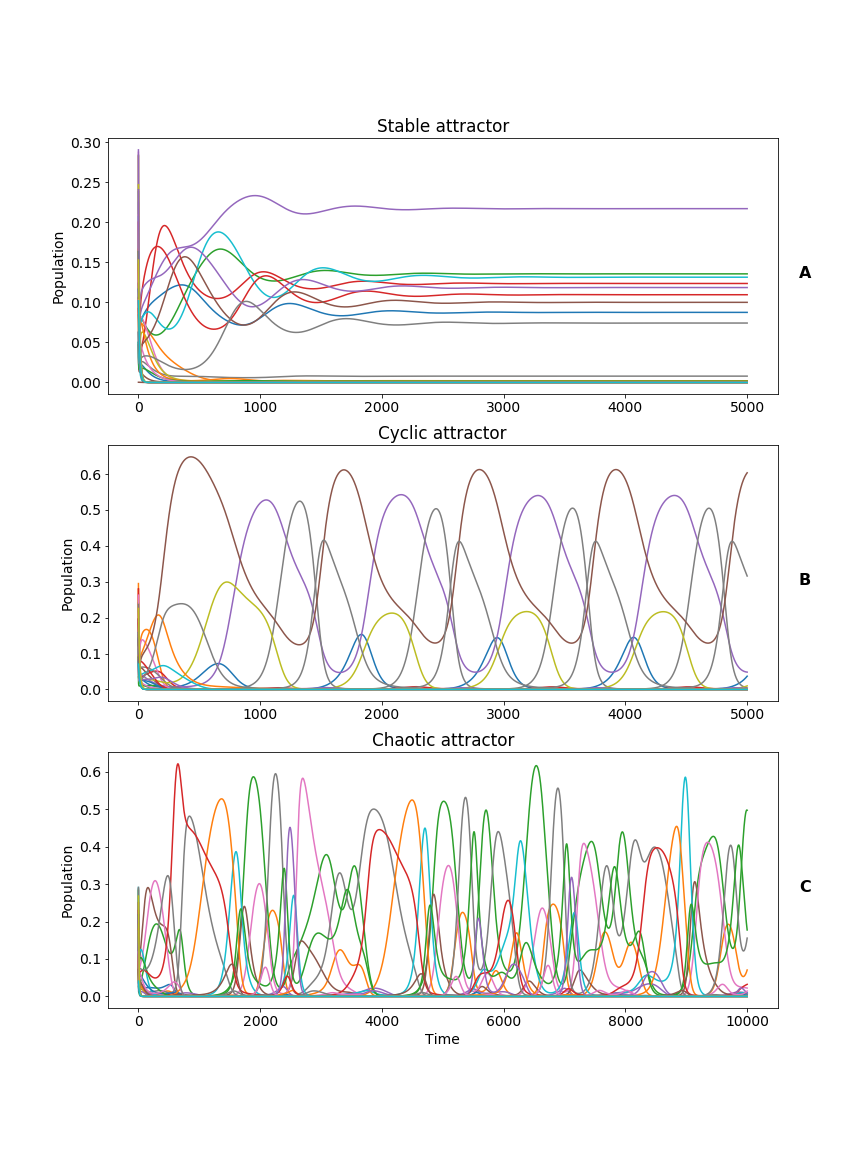
\includegraphics[width=1\columnwidth]{ts.png}
	\end{center}
	\caption{Our model generates time series of the population of each species. The time series can be classified in $3$ types depending on their asymptotic behavior: \textit{stable}, \textit{periodic} and \textit{chaotic}. In \textbf{figure A}, the system reaches a stable attractor after a transient time. In \textbf{figure B}, a periodic attractor, with an approximate period of 1000 days, is reached after the transient time. The system in \textbf{figure C} never reaches a stable nor a cyclic attractor, but a chaotic one.}
	\label{fig:TimeSeries}
\end{figure}

\subsection{Parameterization}
\label{subsec:Parameterization}
For the parameterization of our model we used \cite{Dakos2009b} as a reference. Dakos' model, focusing on plankton communities, uses as well a Rosenzweig-McArthur dynamic with two trophic levels (that of zooplankton and phytoplankton). Unlike Dakos, who uses seasonally changing parameters, our parameters will be constant.

\begin{figure}[H]
	\begin{center}
		\resizebox{\columnwidth}{!}{%
		\begin{tabular}{|c|c|c|c|}
			\hline
			\textbf{Symbol} & \textbf{Interpretation} & \textbf{Value} & \textbf{Units} \\
			\hline
			$r$ & Growth rate & $0.50$ & $d^{-1}$ \\
		    \hline
			$K$ & Carrying capacity & $1.00$ & $ mg \ l^{-1} $ \\
			\hline
			$g$ & Predation rate & $0.40$ & $d^{-1}$\\
			\hline
			$f$ & Immigration rate & $10^{-5}$ & $mg \ l^{-1} \ d^{-1}$\\
			\hline
			$e$ & Assimilation efficiency & $0.60$ & $1$\\
			\hline
			$H$ & Half-saturation constant & $2.00$ & $ mg \ l^{-1} $\\
		    \hline
			$l$ & Loss rate & $0.15$ & $d^{-1}$\\
			\hline
		    $S$ & $ n_C \times n_P $ predator preference matrix & $S_{ij} \sim (0,1)$ & $1$\\
		    \hline
   		    $A$ & $ n_P \times n_P $ competition matrix & See section \ref{subsubsec:CompetitionParameter} & $1$\\
		    \hline
		\end{tabular}}
	\end{center}
	\caption{Values and meanings of the parameters used in our numerical experiment}
	\label{tab:Parameters}
\end{figure}

\subsubsection{Competition parameter}
\label{subsubsec:CompetitionParameter}

%TODO change parameter name
%TODO check parameterization
\todo[backgroundcolor=blue!25]{Change parameter name}
Our aim is to analyze the dynamics of the system described in equation \ref{eq:SystemUnderStudy} for competition interactions differing in heterogeneity. In order to quantify heterogeneity and controlling how far from neutral the competition is, we introduce the competition parameter $ \epsilon $. This dimensionless parameter allows us to vary continuously from interactions where intraspecific competition is stronger than interspecific (for $ \epsilon < 0 $) to the opposite case (for $ \epsilon > 0$). The border between both cases (i.e. $ \epsilon = 0 $), where neither the intra nor the interspecific competition is dominant, represents neutral competition (see figure \ref{fig:CompetitionParameter}).

The numerical implementation of these ideas can be easily achieved by building a competition matrix whose diagonal terms are identically $ 1 $, and whose non-diagonal terms are drawn from a uniform probability distribution centered at $ \epsilon $ and with a given width\todo[backgroundcolor=blue!25]{Mention width somewhere}.

This parameterization allows us to travel continuously from strong dominant intraspecific to strong interspecific competition, meeting neutral competition at the border in between.

\begin{figure}[H]
	\begin{center}
		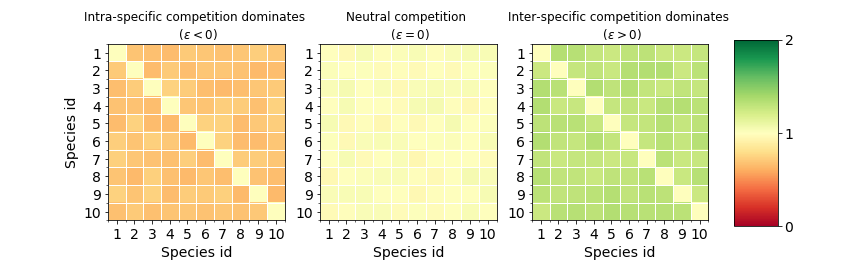
\includegraphics[width=1\columnwidth]{epsilon_all.png}
	\end{center}
	\caption{The competition matrix on the left is a clear case of dominant intraspecific competition. The central one represents a case of neutral competition. The matrix in the right panel shows a case of dominant interspecific competition. The difference between them is the relative size of the non-diagonal elements respective of the diagonal ones. This qualitative property of the competition matrices is controlled by the parameter $\epsilon$.}	
	\label{fig:CompetitionParameter}
\end{figure}

\subsection{Numerical experiment}
\label{subsec:NumericalExperiment}
Our target is to estimate the probability of reaching a chaotic attractor under different degrees of heterogeneity. In order to achieve this, we'll simulate several ecosystems with different initial conditions and relative predation intensities, but sharing the same competition parameter. We consider thus that those ecosystems share a qualitative property: the same degree of heterogeneity. 

Numerical methods are used to integrate the equation \ref{eq:SystemUnderStudy}. A first stabilizing run of $ 2000 $ days is generated in order to get closer to the attractor. Simulating for $ 5000 $ more days, we obtain time series as the ones in figure \ref{fig:TimeSeries}. Using the Gottwald-Melbourne test\cite{Gottwald2009}, we classify each individual simulation as \textit{chaotic} or \textit{non-chaotic}. Our numerical experiment was repeated $ 200 $ times for each competition parameter. The ratio of attractors found to be chaotic can be used to estimate the probability of ecosystems of a given degree of heterogeneity developing chaotic asymptotic behavior.

Additionally, the experiment was repeated for food webs of different sizes. In our simulations, we kept a ratio of 2:3 for the number of species at the consumer and the prey level.

For the sake of reproducibility, we provide a \textit{GitHub} link to the analysis scripts used\footnote{https://github.com/PabRod/Chaos-and-neutrality}\todo[caption={Only footnote}]{Just one footnote. I think it looks nice, but can be integrated in the text if required}.

%Sweeping for different values of $ \epsilon $, we use the following procedure to estimate the probability of a chaotic attractor:
%
%\begin{enumerate}
%	\item Use the competition parameter $ \epsilon $ to draw a competition matrix $ A $ (as described in section \ref{subsubsec:CompetitionParameter}). Notice that this matrix is being drawn from a probability distribution function (PDF), so it will change in every run.
%	\item \label{StartOfAnExperiment} Draw the rest of parameters and initial conditions from the values described in \cite{Dakos2009b}. Those which are defined as ranges will be taken as uniform PDFs. Notice that those parameters taken from a PDF will change in every run.
%	\item Simulate the dynamics numerically.
%	\item Perform two different tests of chaoticity on the simulation (see section \ref{subsec:DetectionOfChaos}).
%	\item Go back to step (\ref{StartOfAnExperiment}) $ R $ times.
%\end{enumerate}

For those more familiar with flow charts, figure \ref{fig:FlowChart} can be illuminating.

\begin{figure}[H]
	\begin{center}
		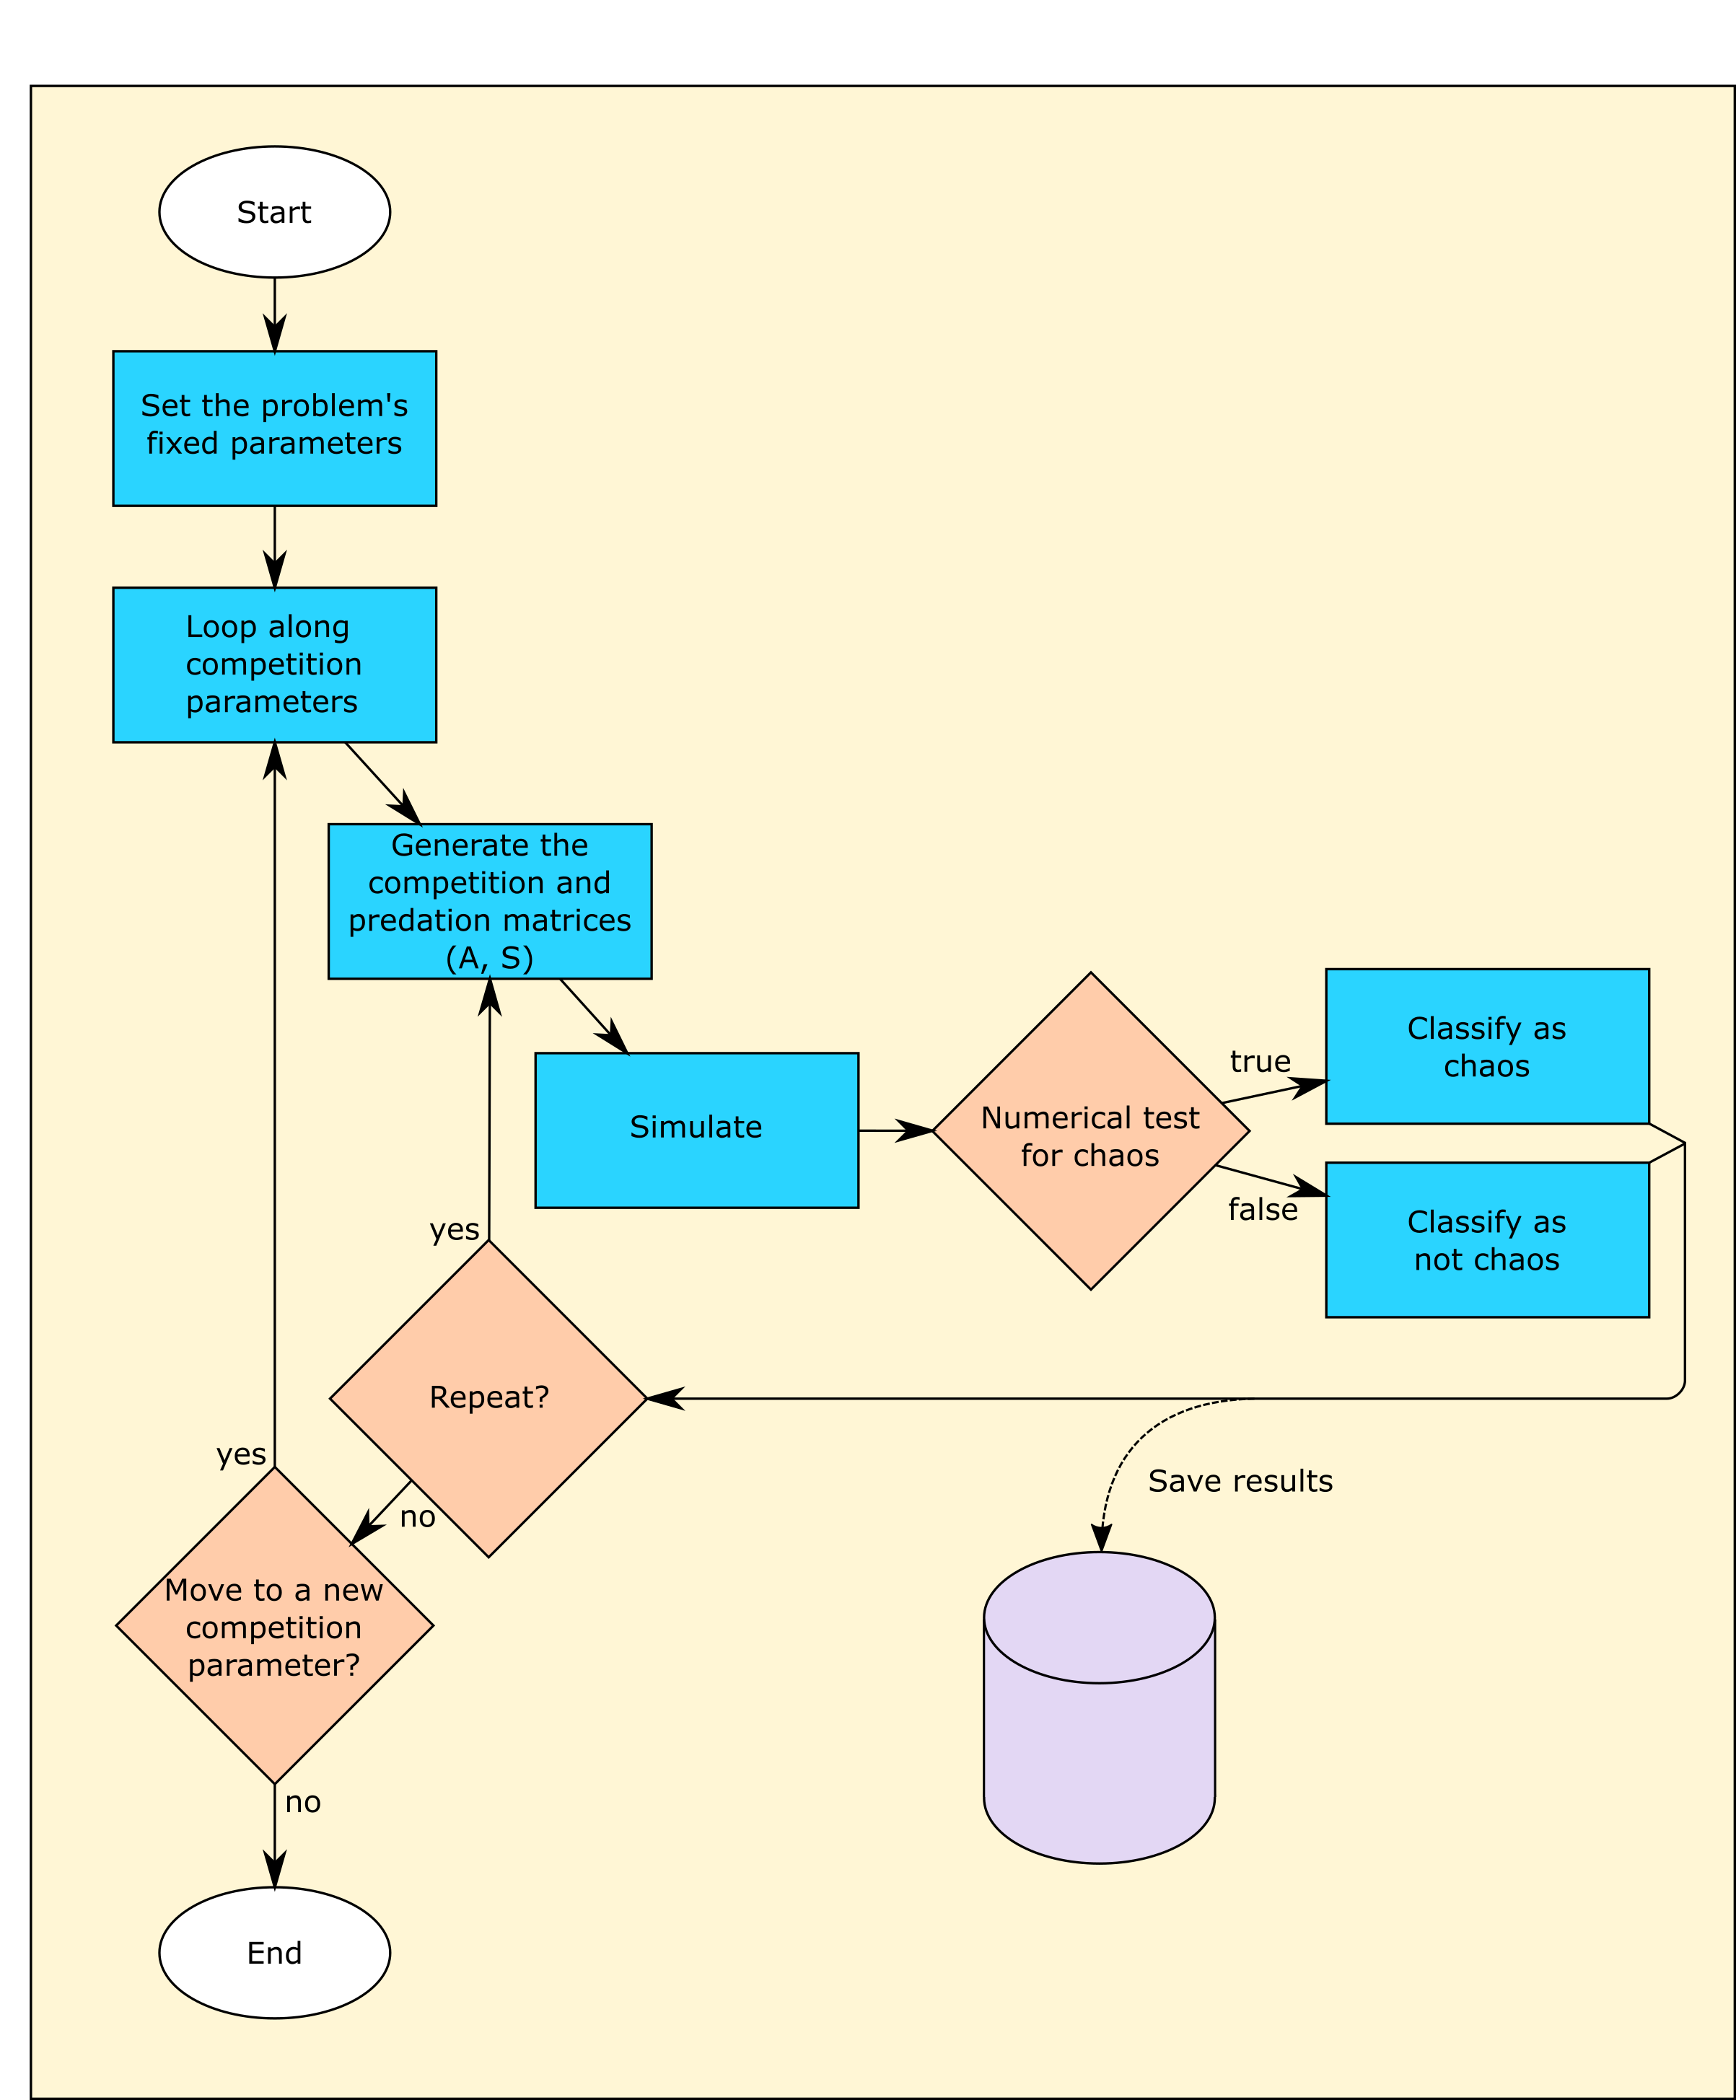
\includegraphics[width=0.9\columnwidth]{flow_chart.png}
	\end{center}
	\caption{Flow chart describing the numerical experiment}
	\label{fig:FlowChart}
\end{figure}

\section{Results}
\label{sec:Results}
Plotting the probability of chaos against the competition parameter (see figures \ref{fig:Results} and \ref{fig:Contour}), we observe a clear maximum around $ \epsilon = 0 $. That is, for neutral competition at the prey's trophic level, the likelihood of chaotic behaviour is higher than for dominant inter or intraspecific competition.

% Weak and strong interspecific competition
There's another local maximum for $ \epsilon = -1 $. This means that ecosystems with weak competition coupling also promote chaos. We consider this a reasonable result, as predation is the driver of chaos.

% Valley
The probability of chaos has a local minimum between $ \epsilon = -1 $ and $ \epsilon = 0 $, whose exact position differs between experiments. We interpret this result as a consequence of the two previous effects: assuming continuity, there should be necessarily at least one local minimum between two local maxima. This is a direct consequence of applying Bolzano's theorem to the first derivative. Intuitively: there should be at least one valley between two mountains.

% Chaos and dimensionality
The overall likelihood of chaos, which can be interpreted as the area under the curve, increases with the size of the food web (see figure \ref{fig:Results}). This effect should not be surprising: the more dimensions the phase space has, the easier is to fulfill the requirements of the complex geometry of a chaotic attractor \cite{Strogatz1994}. We can understand this intuitively as increasing the available room for the trajectories to pack closer and closer without ever crossing each other nor collapsing to a point. Even in those higher dimensional cases, there is still a maximum at neutral competition.

\begin{figure}
	\begin{center}
		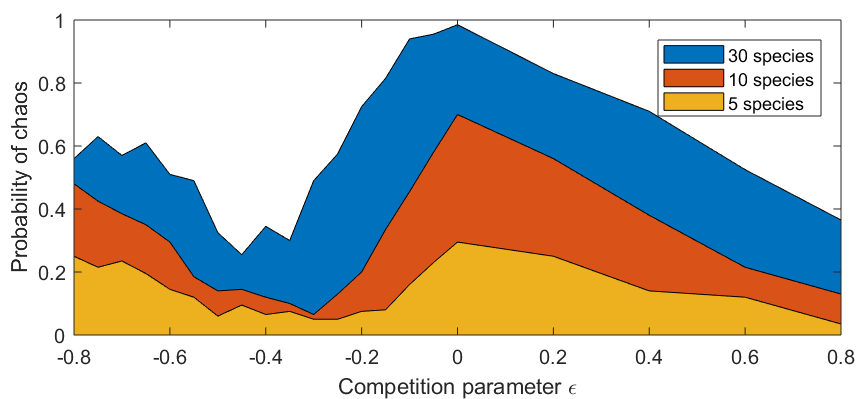
\includegraphics[width=1\columnwidth]{results.png}
	\end{center}
	\caption{Results for a low, medium and high dimensional system. Notice how the probability of chaos has a local maximum around $\epsilon = 0$. The overall probability of chaos, understood as the area under the curve, grows with the system size. The local maximum stays at $\epsilon = 0$ even for systems with a big amount of species.}
	\label{fig:Results}
\end{figure}

\begin{figure}
	\begin{center}
		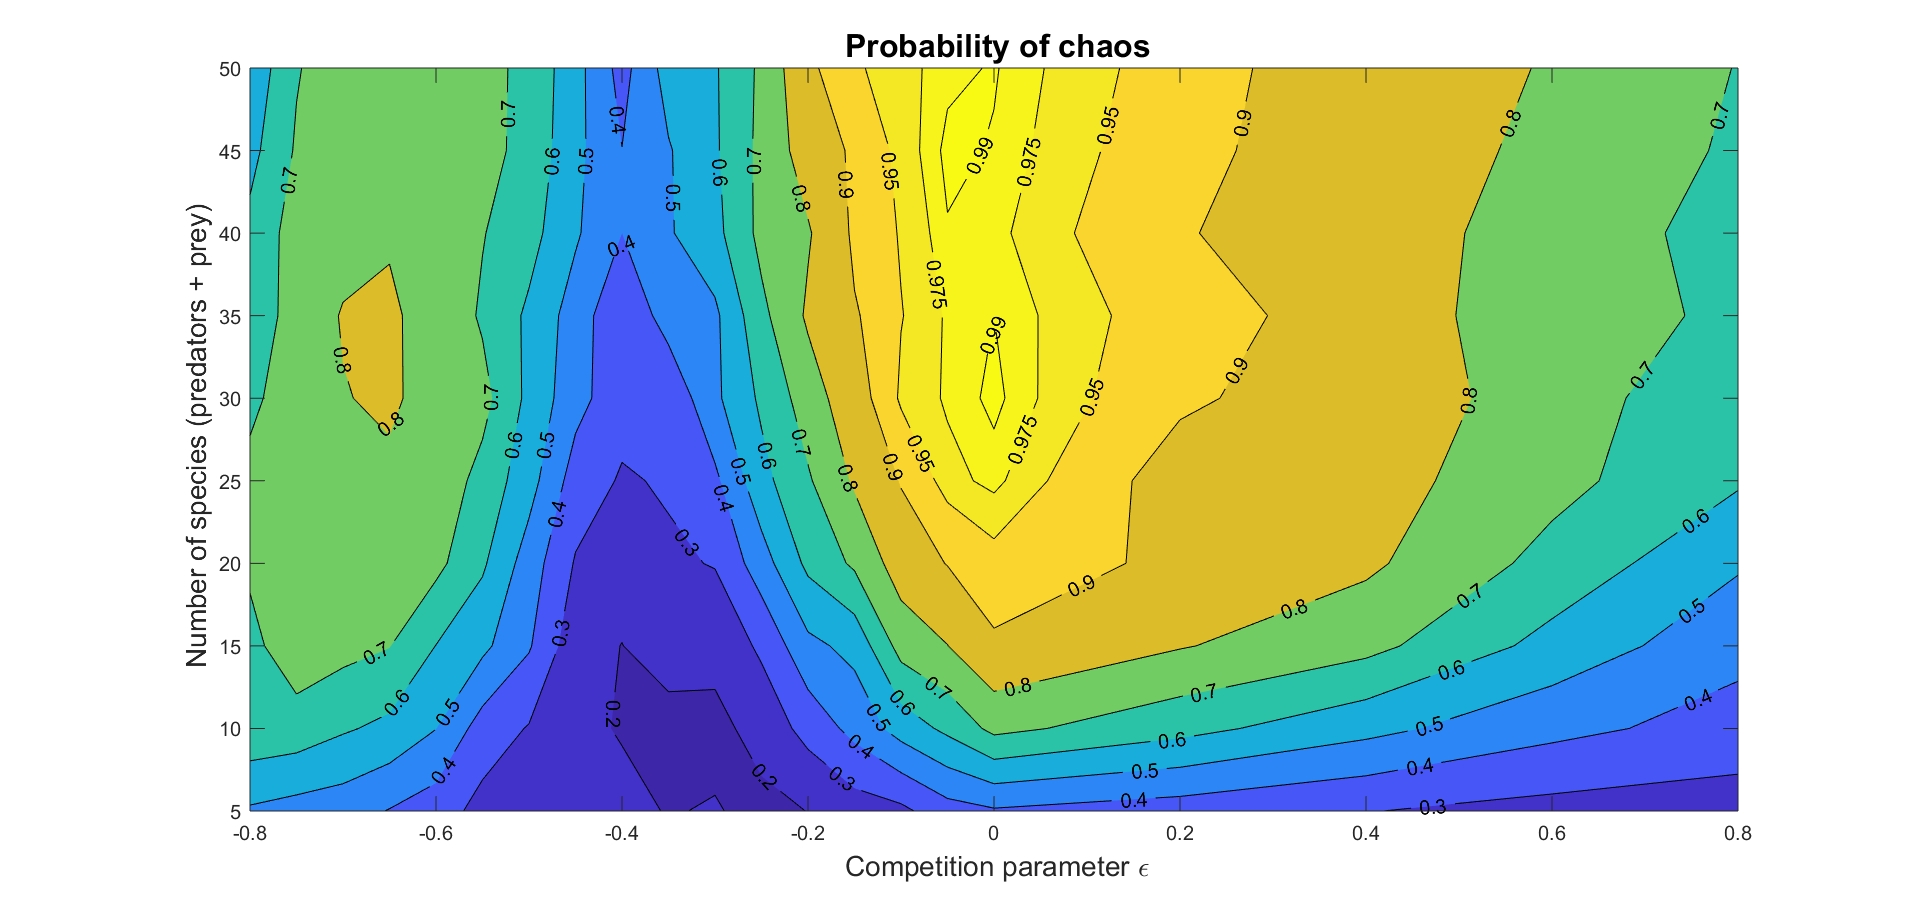
\includegraphics[width=1\columnwidth]{contour.png}
	\end{center}
	\caption{Contour map showing the probability of chaos for various competition parameters (horizontal axis) and prey populations (vertical axis). The consumers' population is fixed as $ 2/3 $ of the prey's population, in order to control the overall size of the system with a single parameter. Notice that chaotic attractors appear more easily (i.e., for smaller systems) the closer is the competition to neutral (i.e., $ \epsilon = 0 $).}
	\label{fig:Contour}
\end{figure}

\section{Discussion}
\label{sec:Discussion} % Our claims
The asymptotic dynamics of our model are affected by the degree of heterogeneity of the competition. Particularly, the closer to neutrality our food web is, the higher are the chances of developing chaotic behaviour. From the biological point of view this observation suggests that the hypothesis of non-equilibrium and Hubbell's hypothesis of neutrality are not completely independent. This suggests that in a system with predation, near-neutrality may increase the probability of non-equilibrium dynamics, increasing the number of coexisting species\todo{Explain a bit more}.
%TODO explain a bit more

% Limitations
In the spirit of mathematical modelling, we chose the simplest realization required for the effects to be observed. We didn't use Allee effect, nor noise, and the functional form of each term has been chosen to account for satiation in the simplest possible way. The choice of a two-level model may seem in contradiction with the pursue of simplicity, but actually it is a fundamental requirement for the effect under research to take place. In the absence of predation, chaos will never develop in a model with neutral competition. The reason for this is that if all interactions become equally strong, the differences among species at the same trophic level fade out. This makes labeling each species meaningless, and thus the prey-only system can be reduced just to one differential equation, that of the total population. Using the Poincar�-Bendixson theorem, it can be proven that chaos cannot be developed in autonomous systems with less than $3$ dimensions\cite{Strogatz1994}.

We used the simplest predation network, that is, one with random prey preference for the predators. A straightforward continuation of this paper could be studying the effect of the type of predation (generalist, specialist, neutral) by choosing other network structures.

% Chaos detection
Numerical detection of chaos has fundamental limitations. There can be boiled down to the fact that, in general, numerical methods cannot distinguish robustly between long transients and genuine chaos. In the present paper three parallel approaches were followed: Lyapunov exponents estimation, Gottwald-Melbourne \textit{0-1} test and visual inspection. Despite differences in the exact probabilities, the three of them led us to the same qualitative conclusions. We found the results of the Gottwald-Melbourne test most consistent with visual inspection. We think that our approach to chaos detection, despite being open to improvement, suffices to hold the biological conclusions.

% The parameter epsilon
Interestingly enough, a relatively small number of replicates suffices to generate a remarkably clear maximum in the probability of chaos for neutral competition. The position of this maximum is independent of the number of interacting species. This suggests that the parameter $ \epsilon $, originally motivated by numerical convenience, may have a biological interpretation by itself. It will be interesting to reverse-engineer this parameter given a set of community matrices validated by experimental or field observations.

% Role of symmetry
It may be worth noting that the position of both the maxima we've found (i.e.: $ \epsilon = -1 $ and $ \epsilon = 0 $) have something in common: the community matrix $ A $ at those values of the parameter is very symmetric in both cases. It will be interesting to develop a similar method that, instead of varying neutrality, varies the less restrictive property of symmetry.

% Is chaos more resilient?
Additionally, we are implicitly assuming without a proof that chaotic ecosystems can have more species than non-chaotic ones\todo{Stronger concluding remark required}.
\todo[inline, caption={This is well known in math}]{There are mathematical reasons for this to be true. Keywords: uniformly hyperbolic dynamical systems, Anosov maps, Arnond's cat map.}
%TODO stronger concluding remark
%TODO there are mathematical reasons for this to be true. Keywords: uniformly hyperbolic dynamical systems, Anosov maps, Arnond's cat map

\todo[inline, caption={Further reading}]{Refer to the discussions about  Huismans paper (Schippers, P., A. M. Verschoor, M. Vos, and W. M. Mooij. 2001. Does "supersaturated coexistence" resolve the "paradox of the plankton"? Ecology letters 4:404-407. and Huismans reply) {Schippers2001}}
%TODO A possible continuation of this research may be the setting of two indepedent ecosystems, one of them chaotic and the other one non-chaotic, and allow them to interact at some point of time (simulating an invasion), in order to assess how much of each of the original ecosystems survives to this traumatic event. This is a good idea, but I think testing for resilience is too far from this study to put it here. You could instead refer to the discussions about  Huismans paper (Schippers, P., A. M. Verschoor, M. Vos, and W. M. Mooij. 2001. Does "supersaturated coexistence" resolve the "paradox of the plankton"? Ecology letters 4:404-407. and Huismans reply) {Schippers2001}

\section{Acknowledgements}
\label{sec:Acknowledgements}
The preliminary analysis of this model were performed using GRIND for Matlab (http://www.sparcs-center.org/grind). Additionally, we thank Jelle Lever, Moussa N'Dour and Sebastian Bathiany for their useful comments and suggestions.

%\clearpage

%\section{Appendix}
%\label{sec:Appendix}
%
%\subsection{Detection of chaos}
%\label{subsec:DetectionOfChaos}
%Dynamical systems with chaotic attractors are extremely sensitive to initial conditions. Two trajectories whose initial conditions are slightly different will diverge exponentially if they lie in the basin of a chaotic attractor. The initial rate of divergence is quantified by the Lyapunov exponent \cite{Strogatz1994}.
%
%Our procedure for classifying the attractors as chaotic or non-chaotic was based in the analysis of Lyapunov exponents. More specifically, this is the procedure we've followed:
%
%\begin{enumerate}
%	\item \label{GoToAttractor} Run the simulation for a sufficient time, in order to guarantee that a trajectory reached an attractor and the dynamics are asymptotic.
%	\item \label{RunInAttractor} Use the last point of the run in step \ref{GoToAttractor} as a starting point for a second, shorter run on the attractor.
%	\item \label{PerturbedTrajectory} Use again the last point of the run in step \ref{GoToAttractor} but, this time, adding a small disturbance to it.
%	\item Compare the runs in steps \ref{RunInAttractor} and \ref{PerturbedTrajectory} to compute numerically the principal Lyapunov exponent.
%	\begin{itemize}
%		\item If it's positive, classify the attractor as chaotic.
%		\item If it's negative, classify the attractor as non-chaotic.
%	\end{itemize}
%\end{enumerate}
%
%\subsection{Neutral competition}
%\label{subsec:NeutralCompetition}
%If we drop everything but the competition part of our dynamics (see equation \ref{eq:SystemUnderStudy}), we will find a system of equations $ n_P $ like the following:
%
%\begin{eqnarray}
%\label{eq:OnlyCompetition}
%\dot{P_i} = P_i \left( 1 - \sum_{k=1}^{n_P} A_{ik} \cdot P_k \right)
%\end{eqnarray}
%
%In order to model a neutral competition, we should use the same competition coefficient for each species. That is, take $ A_{ik} = A $ for all $ i $ and $ k $, so:
%
%\begin{eqnarray}
%\label{eq:OnlyNeutralCompetition}
%\dot{P_i} = P_i \left( 1 - A \sum_{k=1}^{n_P} P_k \right)
%\end{eqnarray}
%
%From equation \ref{eq:OnlyNeutralCompetition} we see that all species have exactly the same dynamical equation. This will make the nullclines to coincide at all points, so the equilibrium points will degenerate to equilibrium manifolds.
%
%\begin{figure}[h]
%	\begin{center}
%		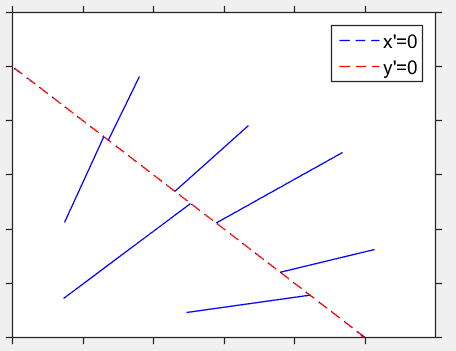
\includegraphics[width=0.9\columnwidth]{degenerate.png}
%	\end{center}
%	\caption{Example with $2$ prey under neutral competition. Both nullclines coincide point to point, giving rise to a higher dimensional equilibirium manifold (in this case, a straight line)}
%	\label{fig:Neutral}
%\end{figure}
%
%This problem can be solved more easily noticing that, from the sole point of view of competition, the effect of neutrality is to fade out the differences between species. Being this the case, the labels $ i $ distinguishing them become pointless. It is a good idea to sum up all the competing species into a new variable, that of total population of (now indistinguishable) species, defined by:
%
%\begin{eqnarray}
%\label{eq:TotalPopulation}
%	T(t) = \sum_{i=1}^{n_P} P_i(t)
%\end{eqnarray}
%
%It can be shown using equation \ref{eq:OnlyNeutralCompetition} that, as expected from the biological intuition, the dynamics of this new variable will follow the same differential equation as the individual species abundances. This collapses the $ n_P $ dimensions of our original problem to a single one.
%
%\begin{eqnarray}
%\label{eq:TotalPopulationDynamics}
%	\dot T(t) = \sum_{i=1}^{n_P} \dot P_i(t) = T (1 - A T)
%\end{eqnarray}
%
%In our model, the predation interaction breaks this excess of symmetry, so we can still work with neutral competition as long as the predation is not neutral without facing problems of system degeneration.

\clearpage

\bibliography{library}
\bibliographystyle{vancouver}

%\listoftables
%\listoffigures

%TODO
\todo[inline, backgroundcolor=blue!25, caption={Citation style}]{Do we want to keep the 'Available from + URL' structure in the bibliography?}
%TODO Create an online appendix with extra figures, different chaos tests, different random distributions
\todo[inline, caption={Online appendix}]{Create an online appendix with extra figures, different chaos tests, different random distributions}
%TODO Double check figures
\todo[inline]{Double check figures}

\end{document}